% !TEX root = ./summary.tex

\section{Einrichten von \antlr auf Eclipse}
In diesem Kapitel geht es darum \antlr herunter zu laden, um es danach in Eclipse zu integrieren. 

\subsection{Schritt 1 - \antlr herunterladen}
\label{sec:step1}
\antlr von \href{http://www.antlr.org/download}{http://www.antlr.org/download} herunterladen. Am besten nimmt man dazu die \textbf{antlr-X.X.X-complete.jar}. Wenn die Source Attachments unbedingt eingesehen werden mu"ssen, kann auch noch das .zip u"ber \href{http://www.antlr.org/download.html}{http://www.antlr.org/download.html} heruntergeladen werden.\\
\textbf{Es ist wichtig diese Dateien irgendwo abzulegen, wo sie immer wieder gefunden werden k"onnen.}

\subsection{Schritt 2 - \antlr Plugin installieren und einrichten}
F"ur \antlr gibt es ein Plugin, welches sich leicht auf dem Eclipse Marketplace finden l"asst. Man muss dazu einfach \antlr in dessen Suche eingeben und dann auf installieren klicken.

\begin{figure}[H]
	\centering
	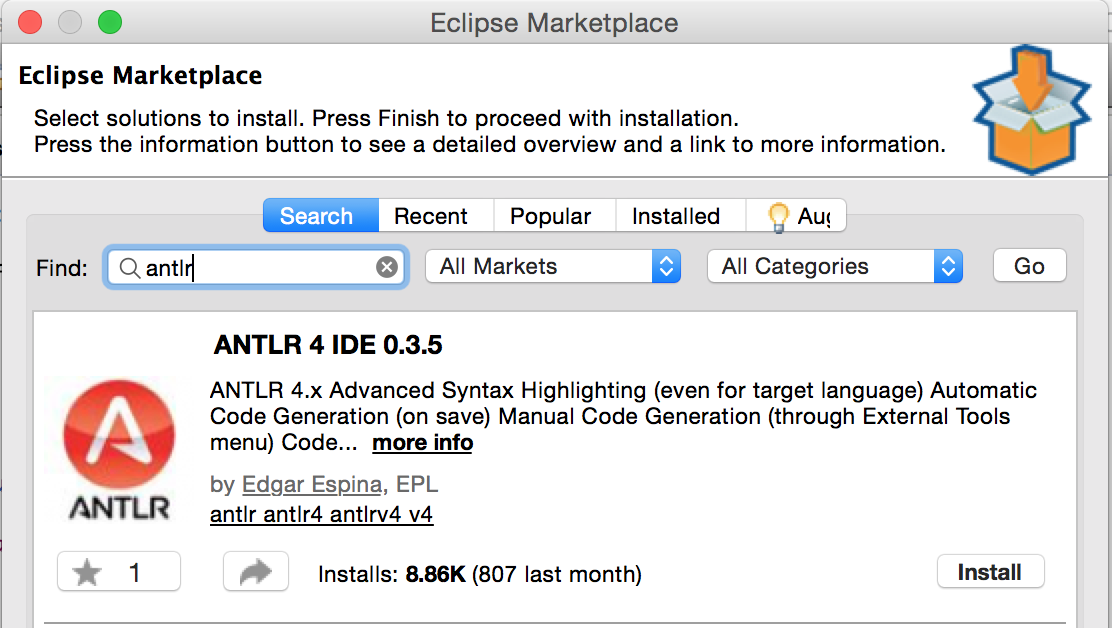
\includegraphics[width=0.65\textwidth]{antlr_plugin}
	\caption{\antlr Plugin im Eclipse Marketplace}
\end{figure}

Als n"achstes muss das Plugin noch eingerichtet werden. 

\begin{figure}[H]
	\centering
	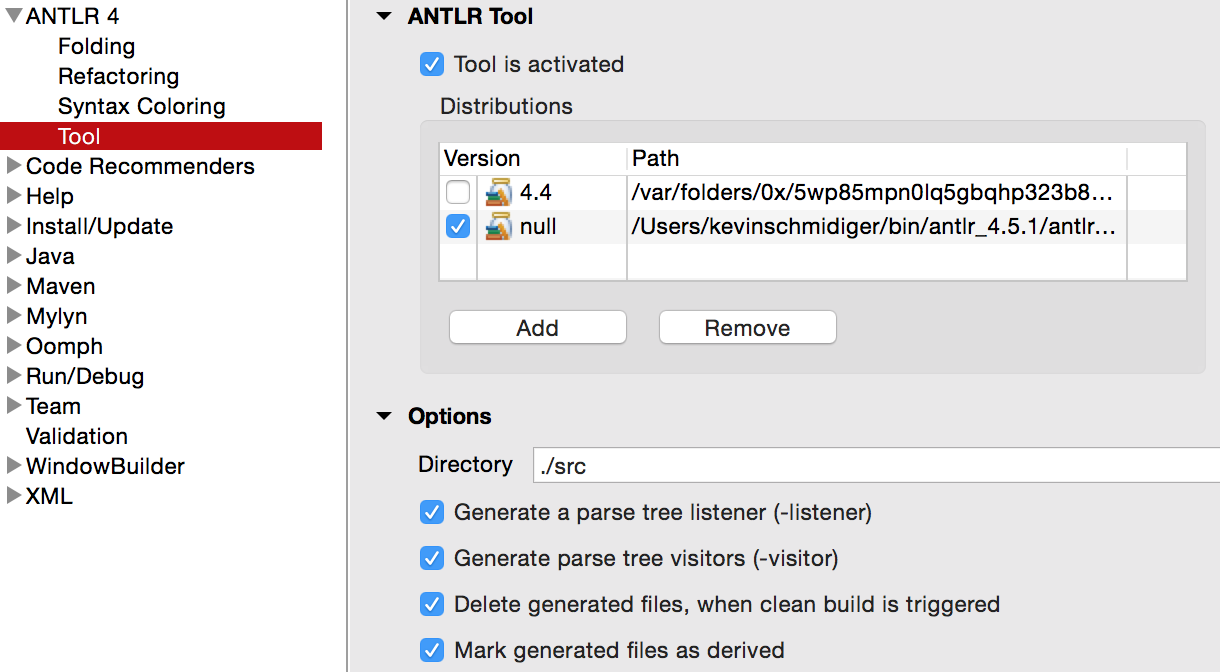
\includegraphics[width=0.65\textwidth]{antlr_config}
	\caption{\antlr Konfigurationsmenu}
\end{figure}

Es ist zu beachten, dass das Directory ge"andert wird zu ./src. Das ist der Ausgabeort von dem von \antlr generiertem Code. Auch w"urde ich die default Version wechseln zu der, die in Kapitel~\ref{sec:step1} heruntergeladen wurde. 

\subsection{Schritt 3 - Projekt aufsetzen}
Ein neues Projekt aufsetzten ist nicht schwirig. Man muss nur ein normales Java Projekt erstellen und eine gewisse Ordnerstruktur einhalten. 